\documentclass[12pt]{article}

\usepackage[a4paper, total={7in, 9in}]{geometry}
\usepackage{graphicx}
\graphicspath{ {./images/} }
\usepackage{algorithm}
\usepackage{algorithmic}
\usepackage{hyperref}

\setlength{\footskip}{50pt}

\begin{document}
\title{\vspace{-3cm}Reader Info Method}
\author{Ben Duggan}
\date{\today}
\maketitle

\section{General notes}
\begin{itemize}
	\item You will need to use node.js when running this code.  Download it from online. To run the website code navigate to the server folder.  Then type \textit{npm install express mysql socket.io winston} to install the server dependences.  You only have to do that step the first time.  Next run the application by typing \textit{node index}.  You will see some errors about connecting to MySQL DB but ignore those.  Navigate to \textit{localhost:4000} on your web browser and go to the Readers page.  This is where you're working.
\end{itemize}

\section{Goal}
The goal is to create a network diagram of the radios used.  The radios store the tree in an array with elements having a nodeID, unique id, and address, the address of the radio.  The tree is a 5-arry tree with an address of 0 being the master node (Raspberry Pi).  The address represents the path to get from itself to master.  Addresses have the following rules (from \url{http://tmrh20.github.io/RF24Network/}):
\begin{itemize}
	\item Node 00 is the base node.
	\item Nodes 01-05 are nodes whose parent is the base.
	\item Node 021 is the second child of node 01.
	\item Node 0321 is the third child of node 021, an so on.
	\item The largest node address is 05555, so up to 781 nodes are allowed on a single channel. An example topology is shown below, with 5 nodes in direct communication with the master node, and multiple leaf nodes spread out at a distance, using intermediate nodes to reach other nodes.
\end{itemize}
The main goal is to create an enhanced, dynamic and responsive table similar to this one from \url{http://tmrh20.github.io/RF24Network/}:\\
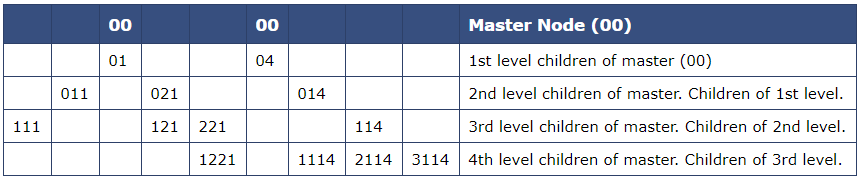
\includegraphics[width=6in]{example_table}\\

\section{Implementation}
All of your code will be implemented in readers.js which is found in server/dependences on the GitHub repo, \url{https://github.com/BenSDuggan/RFID-Network}.  You will add all of your code to the createMeshTable() method in that file.  The method takes an argument addrList which is an array of JSON objects where each element is a readers information.  The key-value pairs that you care about are "id" which is the nodeID and "address" which is the address.\\

You will be making a HTML table to represent the network tree.  The data is inserted into a table with id "reader-MNC".  This means that you just have to write the internal HTML (append this to 'content').  You shouldn't have to touch much CSS as that is handled by BootStrap.  A good reference on HTML tables is from \href{https://www.w3schools.com/html/html_tables.asp}{W3 Schools}.\\

The actual data is stored in readers.json in server/RFIDNetworkPi.  The sample data in there is but you can add your own test data.\\

\section{ToDos}
\begin{enumerate}
	\item Take addrList and add all data to HTML table, ignoring responsiveness and style, similar to the table above but without the description of each level.  Here are some recommended sub-goals.
	\begin{enumerate}
		\item First create a new array (or JSON) variable used to store the nodes the level of each element from addrList.  This can be achieved by casting "address" to a string and getting the length.
		\item Next iterate over each level of that array using a for loop.  During each iteration organize the elements inorder, create a new row and add the id and address to the table.
	\end{enumerate}
	This should give you something similar to the table above.
	\item Edge cases.  There are two edge cases: when the address is 0 and when its "".  Both cases mean that the node is not in the tree but was once there.  Add the ids of these nodes to the div with id="reader-deadNodes".  Again you can just append to content in the later part of the method.  Here are some recommended subgoals:
	\begin{enumerate}
		\item Before adding any data to the table (because we don't want dead nodes in the table), create a new array, iterate through addrList, add elements with address==0 || address=="" to the new array and remove them from addrList.
		\item Iterate through that array and append them to content.
	\end{enumerate}
	\item Add color.
\end{enumerate}



\end{document}

